\documentclass[10pt,utf8]{beamer}

\mode<presentation> {
%  \usetheme{Boadilla}
  \usetheme{Madrid}
%	\usetheme{Fzu}
  \setbeamercovered{transparent}
}

\usepackage{palatino}
\usepackage{graphicx}
\usepackage{array}
\usepackage{color}
\usepackage{subfigure}
\usepackage{colortbl}
\usepackage{amsmath}
\usepackage{hyperref}


\setbeamertemplate{caption}{\raggedright\insertcaption\par} %turn off caption prefix ("Figure")

\title{RAFT}
\author{Vojtech Juranek}
\institute[Red Hat]{JBoss - a division by Red Hat}
\date{CHANGE ME: date, RH internal, Brno}


\begin{document}

\begin{frame}
 \titlepage
\end{frame}


\begin{frame}
  \frametitle{Outline}
  \begin{itemize}
    \item Leader election
		\item Log replication
		\item Membership changes
  \end{itemize}
\end{frame}


\begin{frame}
  \frametitle{General properties}
	\begin{itemize}
		\item Algorithm for implementing replicated log (replicated state machine - all nodes execute commands in the same order)
		\item Can work only as long as majority of nodes is responding
		\item CP
		\item Strong leadership (log entries flow only from leader to other entries)
	\end{itemize}
\end{frame}

\begin{frame}
	\frametitle{How Raft works}
	\begin{figure}
		\centering
		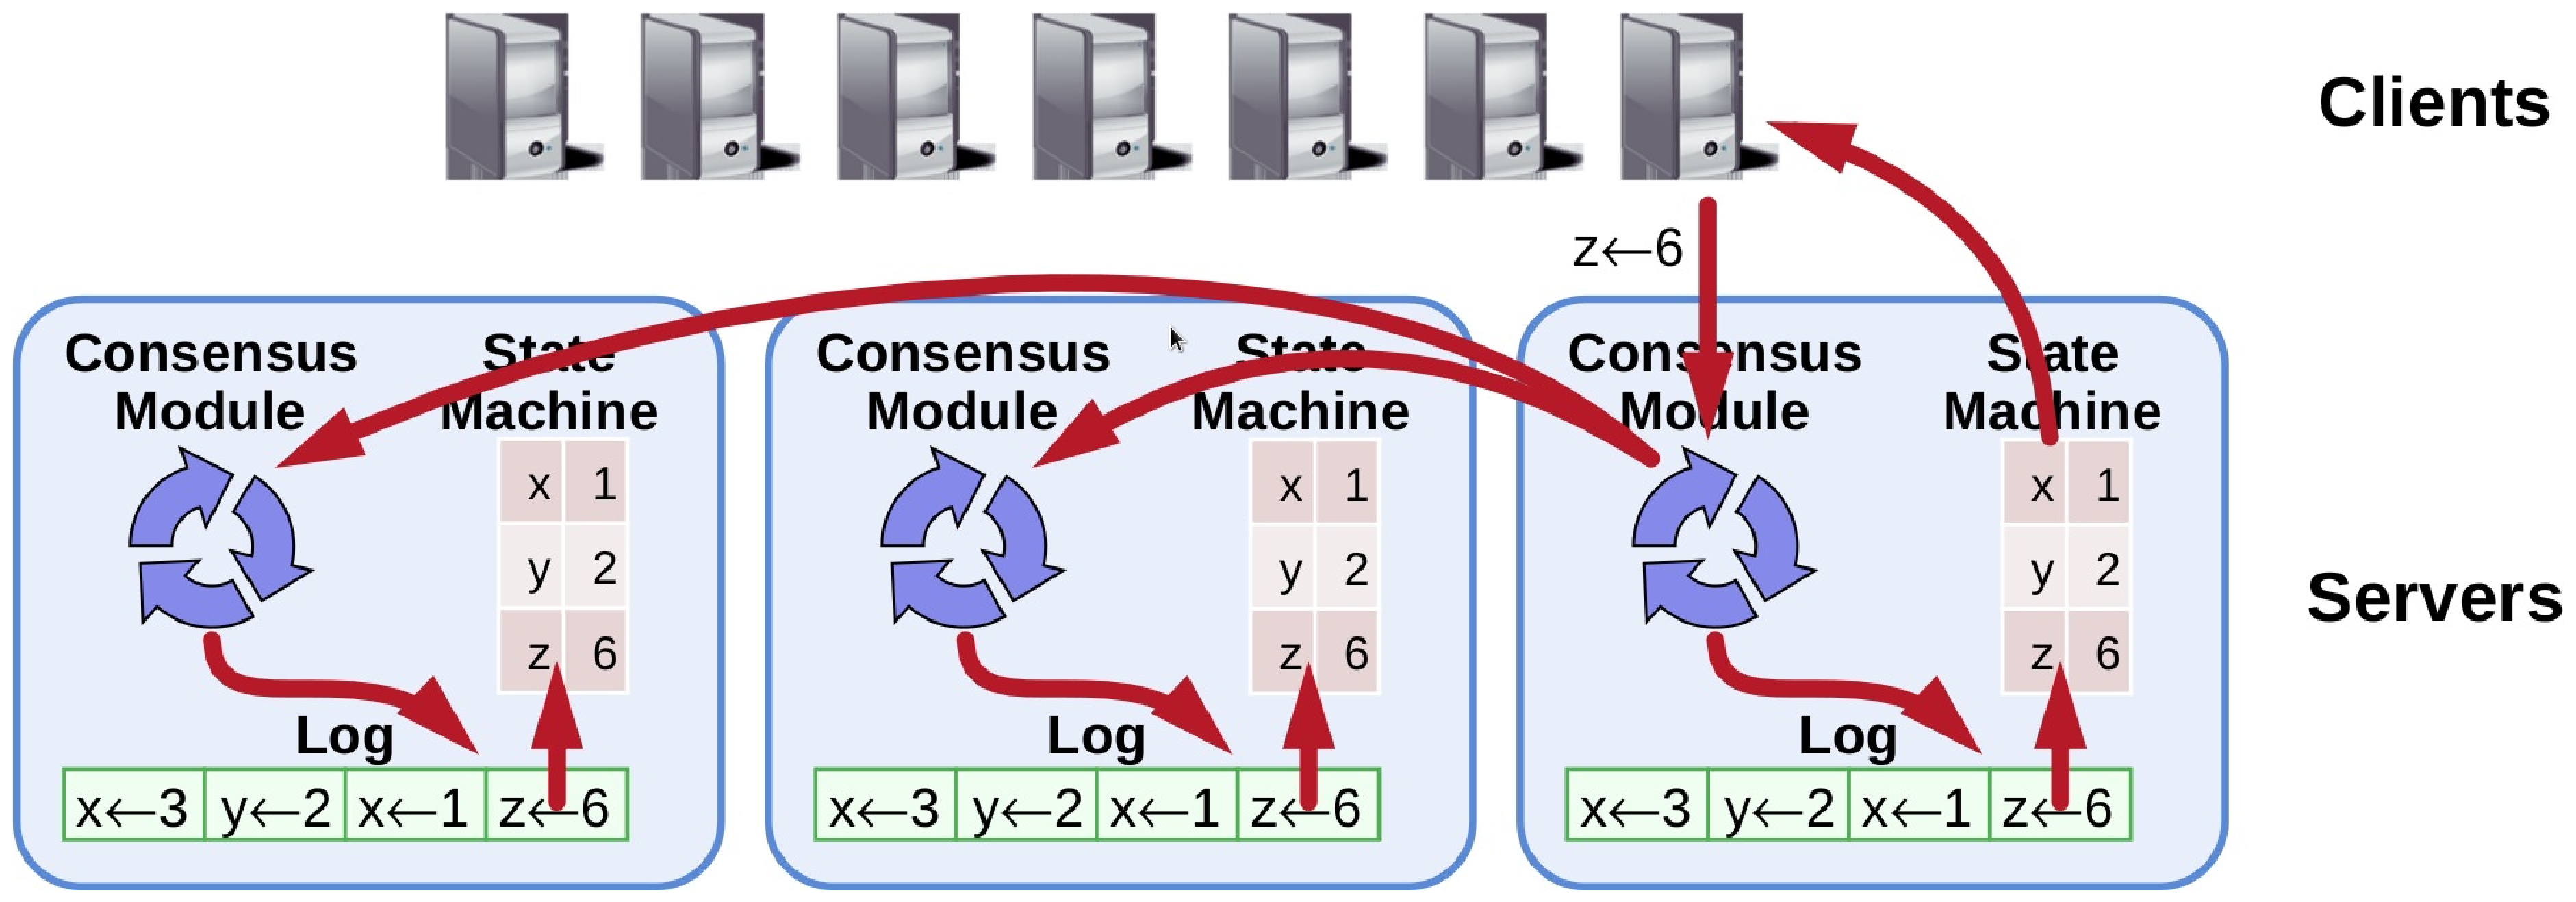
\includegraphics[width=12cm]{./img/log_repl.eps}
		\caption{\tiny{Source: \url{https://raft.github.io/slides/rustdiego2015.pdf}}}
	\end{figure}
	\begin{itemize}
		\item A leader is elected.
		\item Leader has complete responsibility to maintain the log.
		\item Only leader accepts client requests.
		\item Leader replicates entries submited by clients to other servers.
		\item Leader notifies other server when it's safe to apply new entries to their state machines.
	\end{itemize}
\end{frame}


\begin{frame}
	\frametitle{Server states}
	\begin{figure}
		\centering
		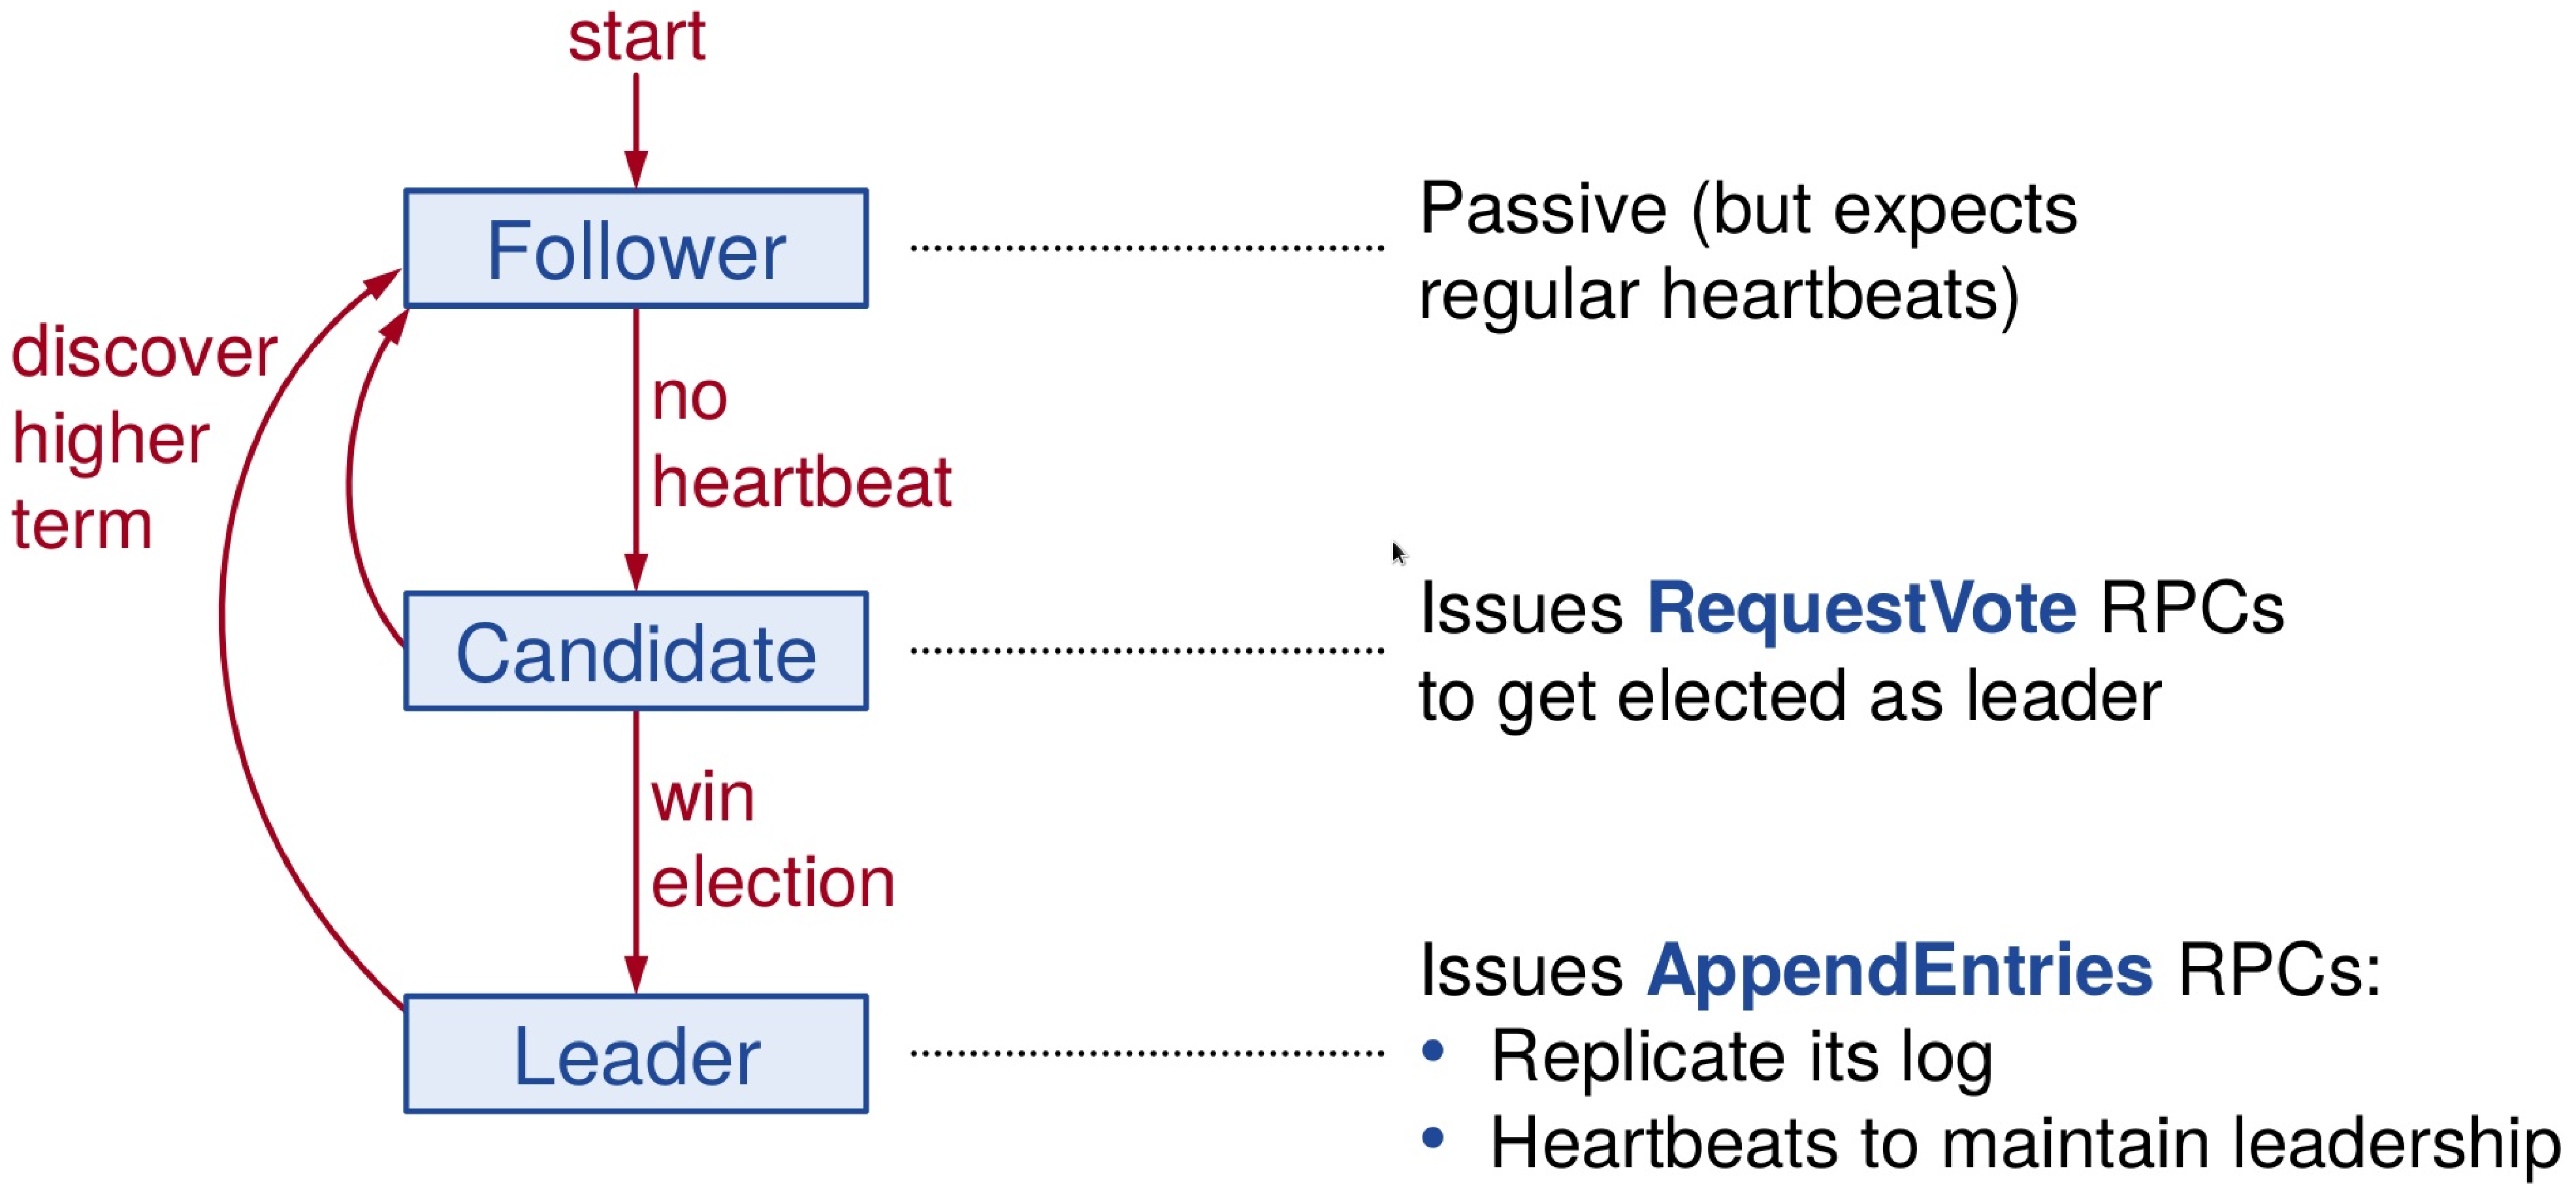
\includegraphics[width=12cm]{./img/server_states.eps}
		\caption{\tiny{Source: \url{https://raft.github.io/slides/uiuc2016.pdf}}}
	\end{figure}
\end{frame}


\begin{frame}
	\frametitle{Leader election}
	\begin{figure}
		\centering
		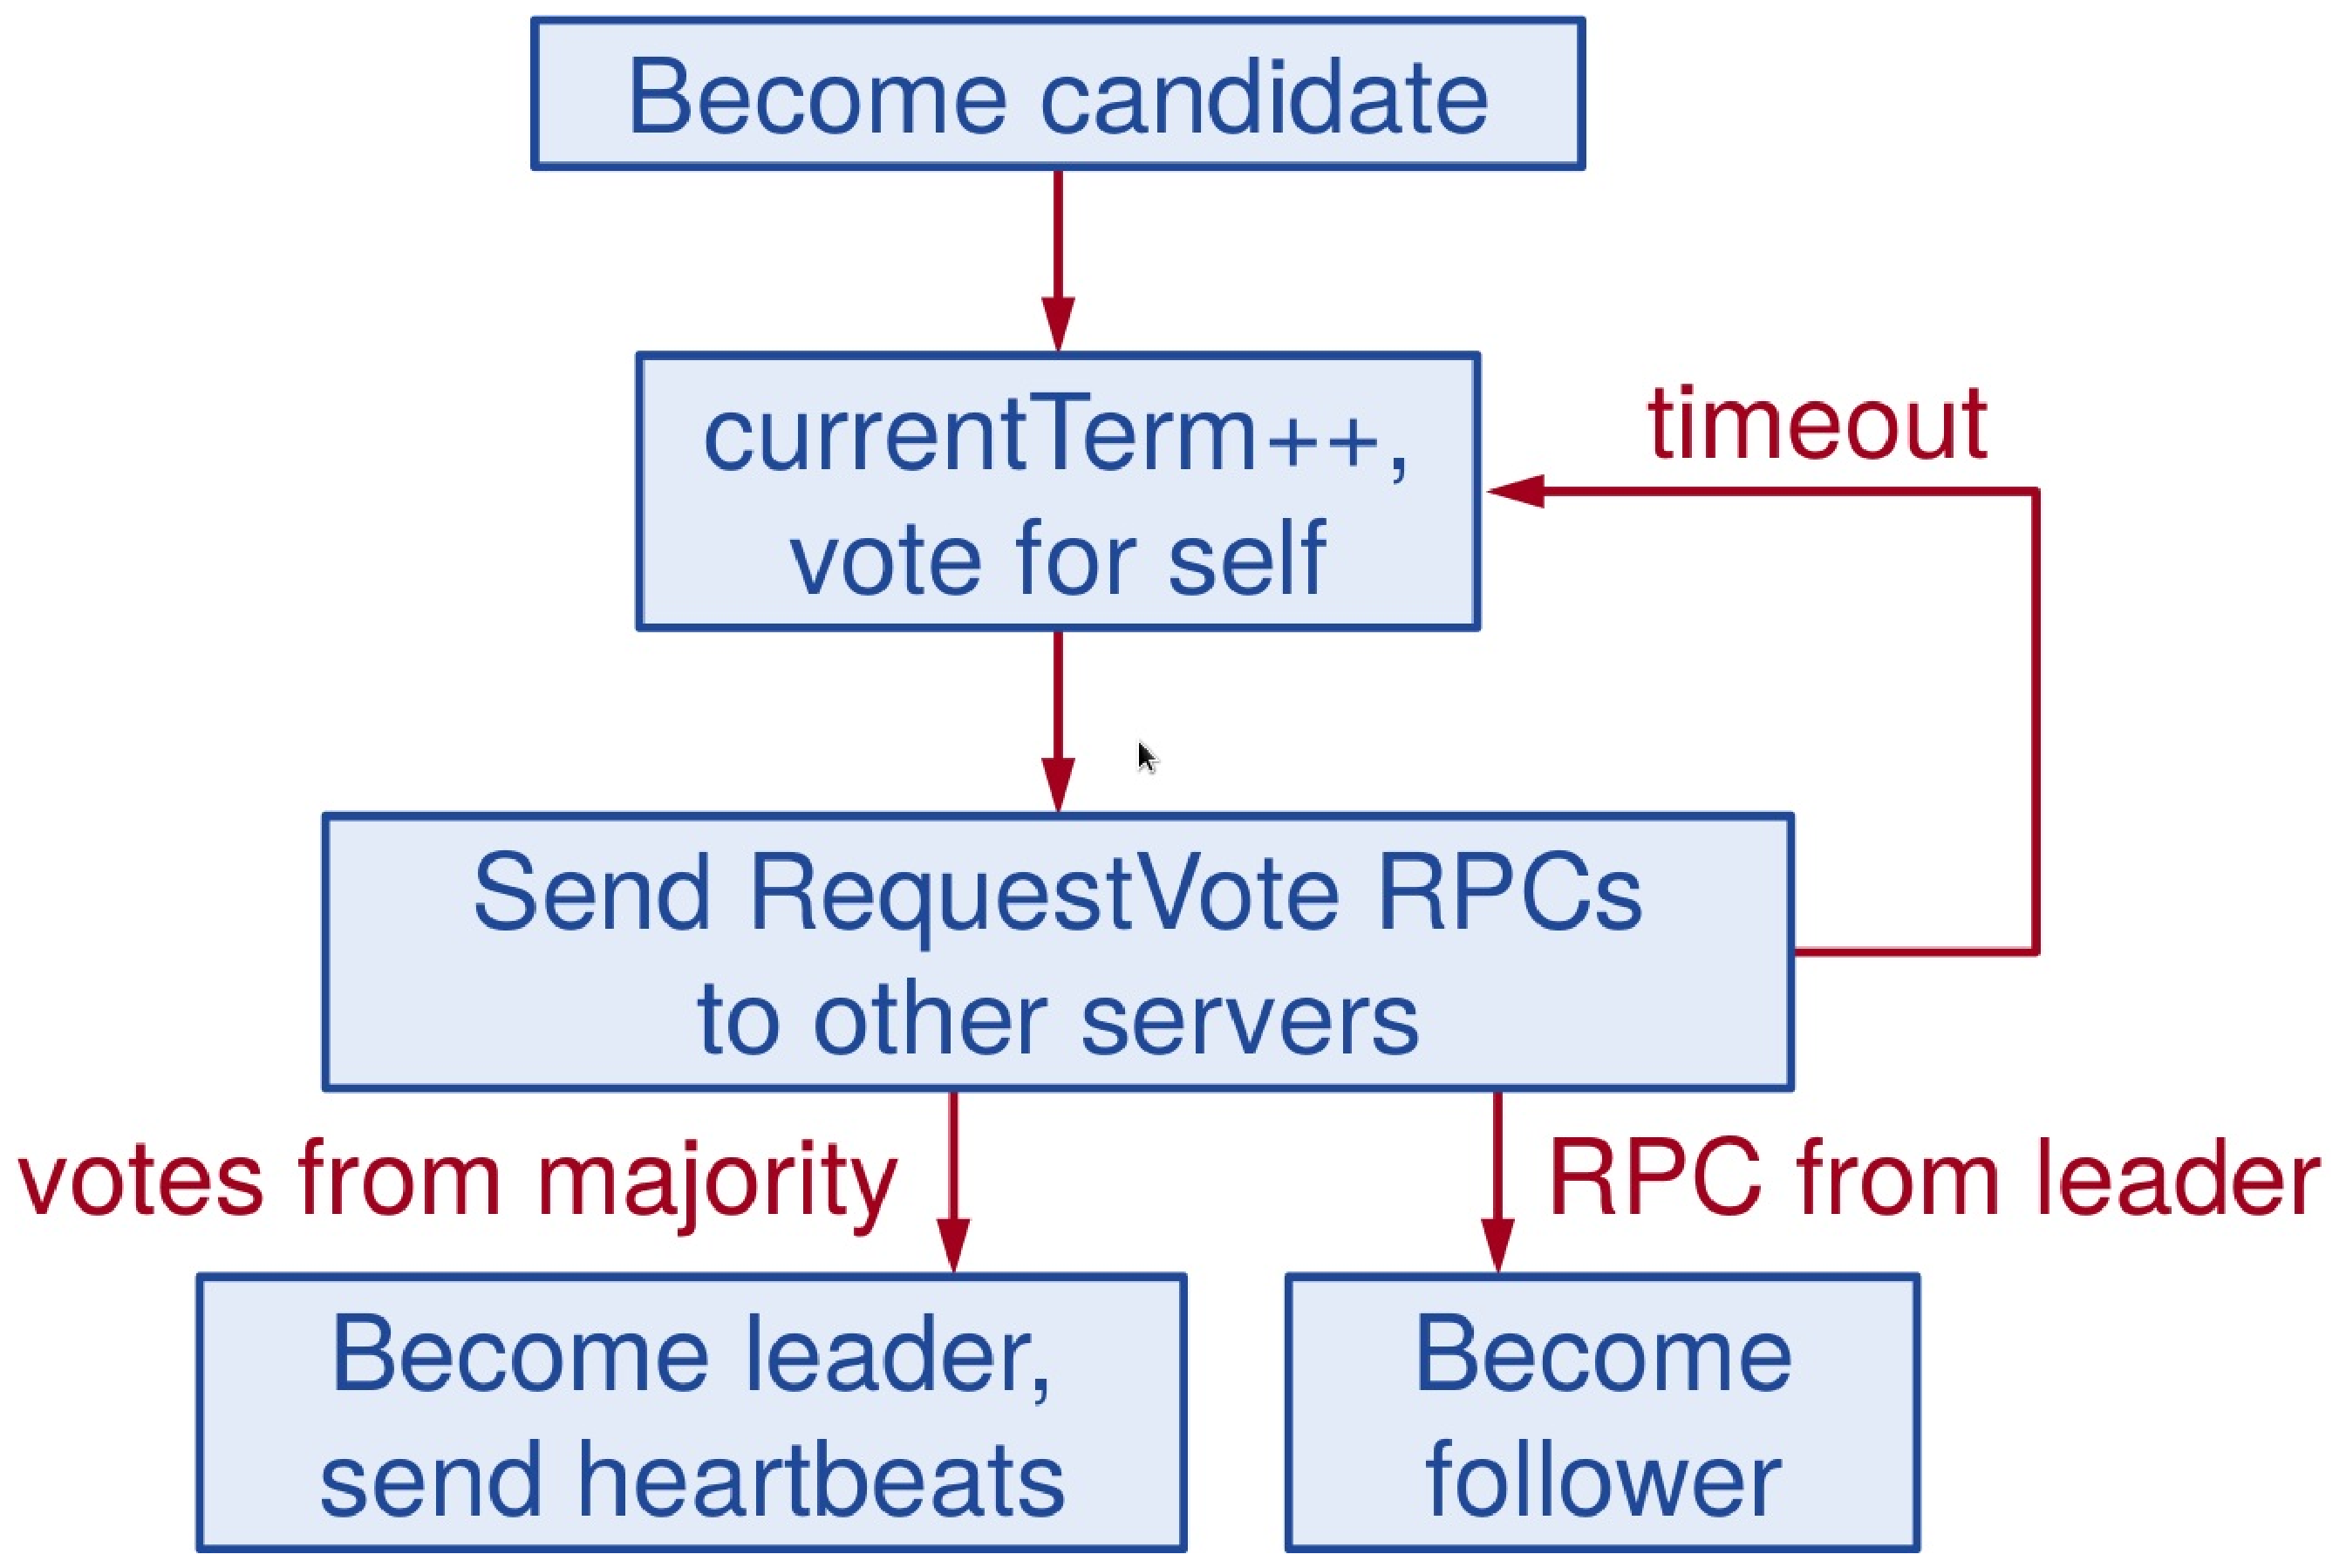
\includegraphics[width=10cm]{./img/leader_election.eps}
		\caption{\tiny{Source: \url{https://raft.github.io/slides/uiuc2016.pdf}}}
	\end{figure}
\end{frame}


\begin{frame}
	\frametitle{Log structure}
	\begin{figure}
		\centering
		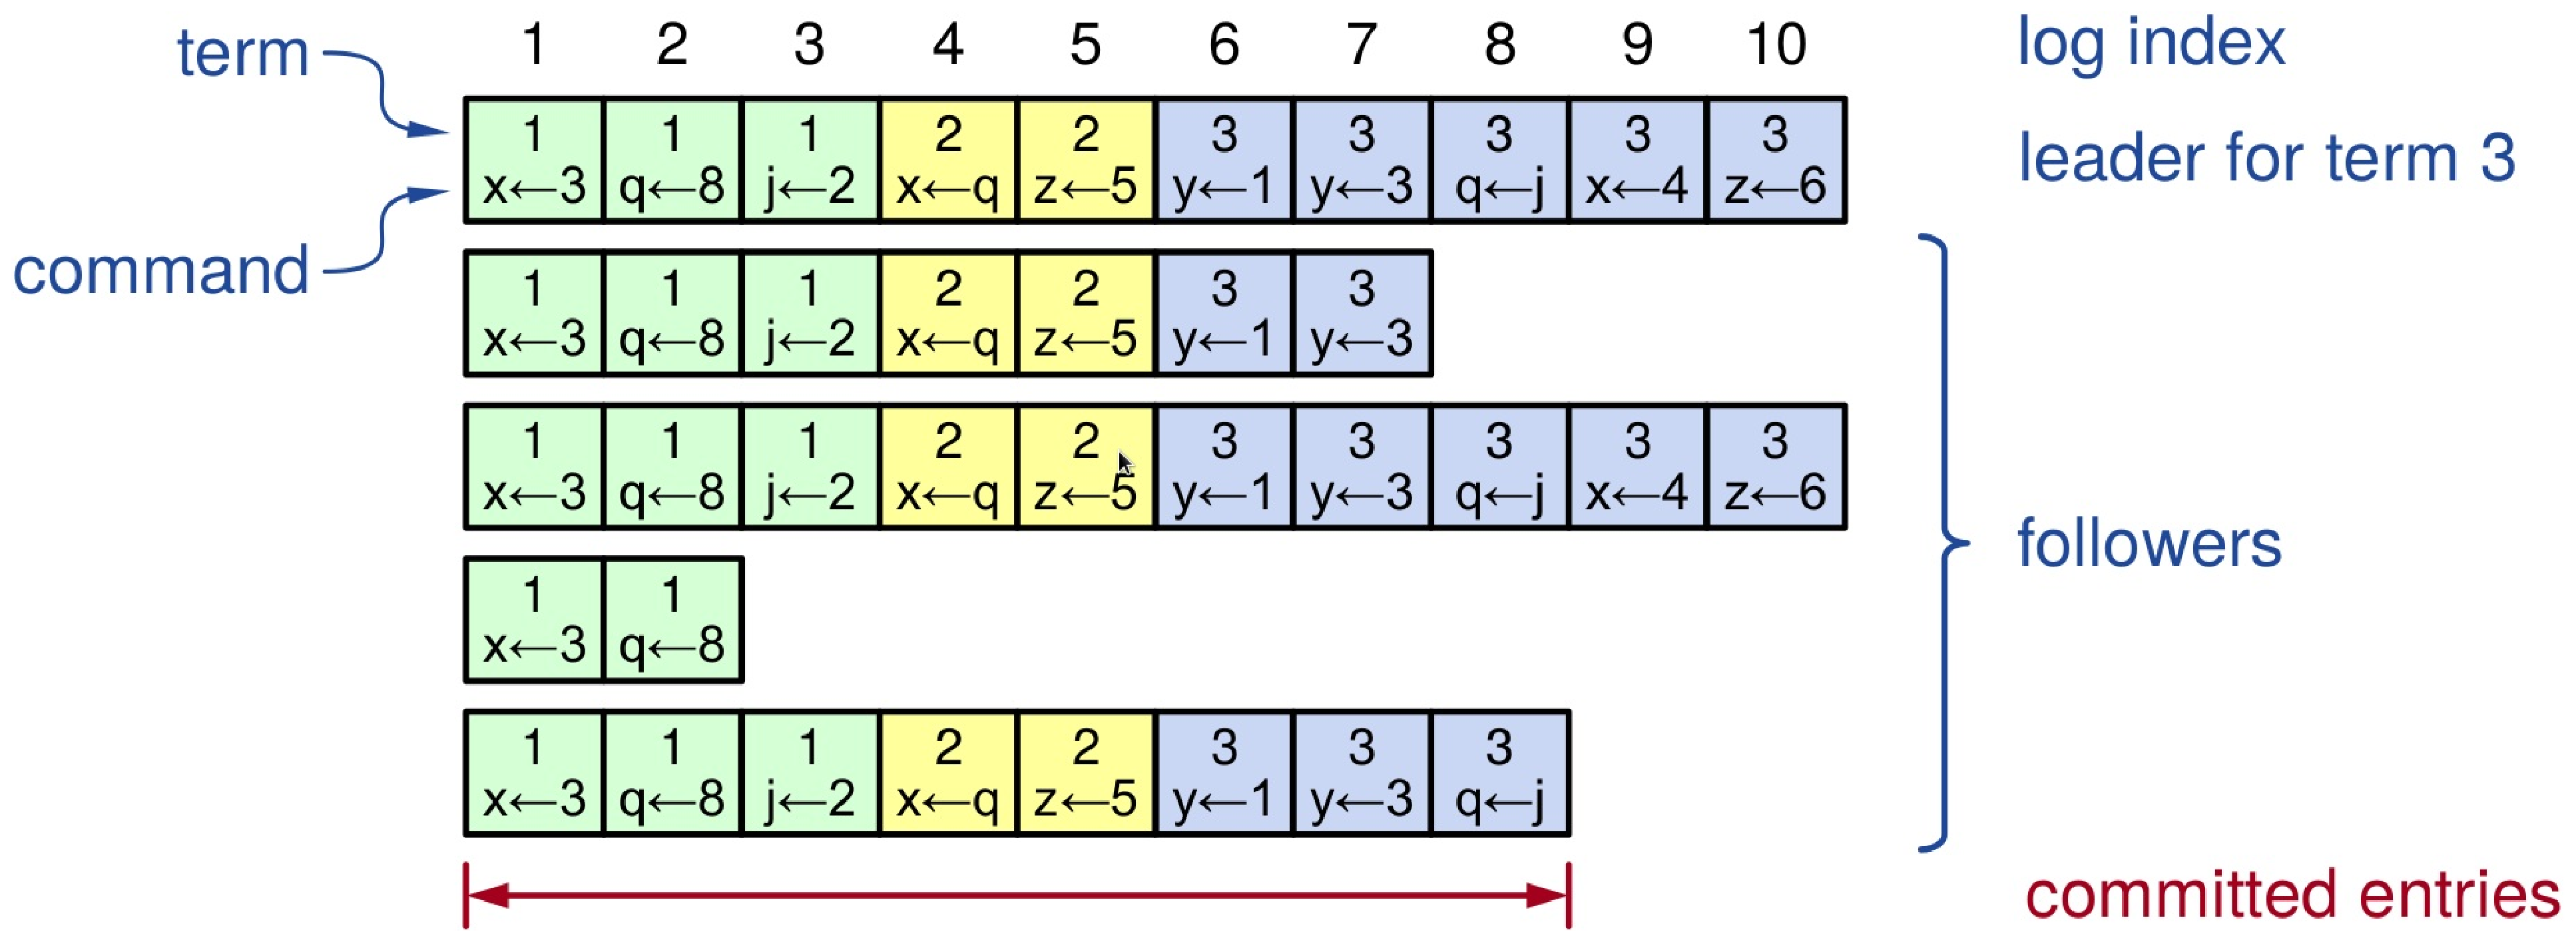
\includegraphics[width=12cm]{./img/log_structure.eps}
		\caption{\tiny{Source: \url{https://raft.github.io/slides/uiuc2016.pdf}}}
	\end{figure}
\end{frame}


\begin{frame}
	\frametitle{Log replication}
	\begin{itemize}
		\item Command can complete as soon as majority of the cluster resposnded.
	\end{itemize}
\end{frame}


\begin{frame}
	\frametitle{References}
	\begin{thebibliography}{9}
		\bibitem{raft_paper} \url{https://raft.github.io/raft.pdf}
	\end{thebibliography}
\end{frame}


\end{document}